\section{Training Behavior}
\label{sec:training}

Figure~\ref{fig:training} plots the SFT run and both DPO runs. The training curves are noisy, because each point comes from a single batch of 32, so I judge convergence from the validation measurements: 1,000 held-out examples for SFT and 1,000 held-out preference pairs for each DPO run.

\begin{figure}[!t]
\centering
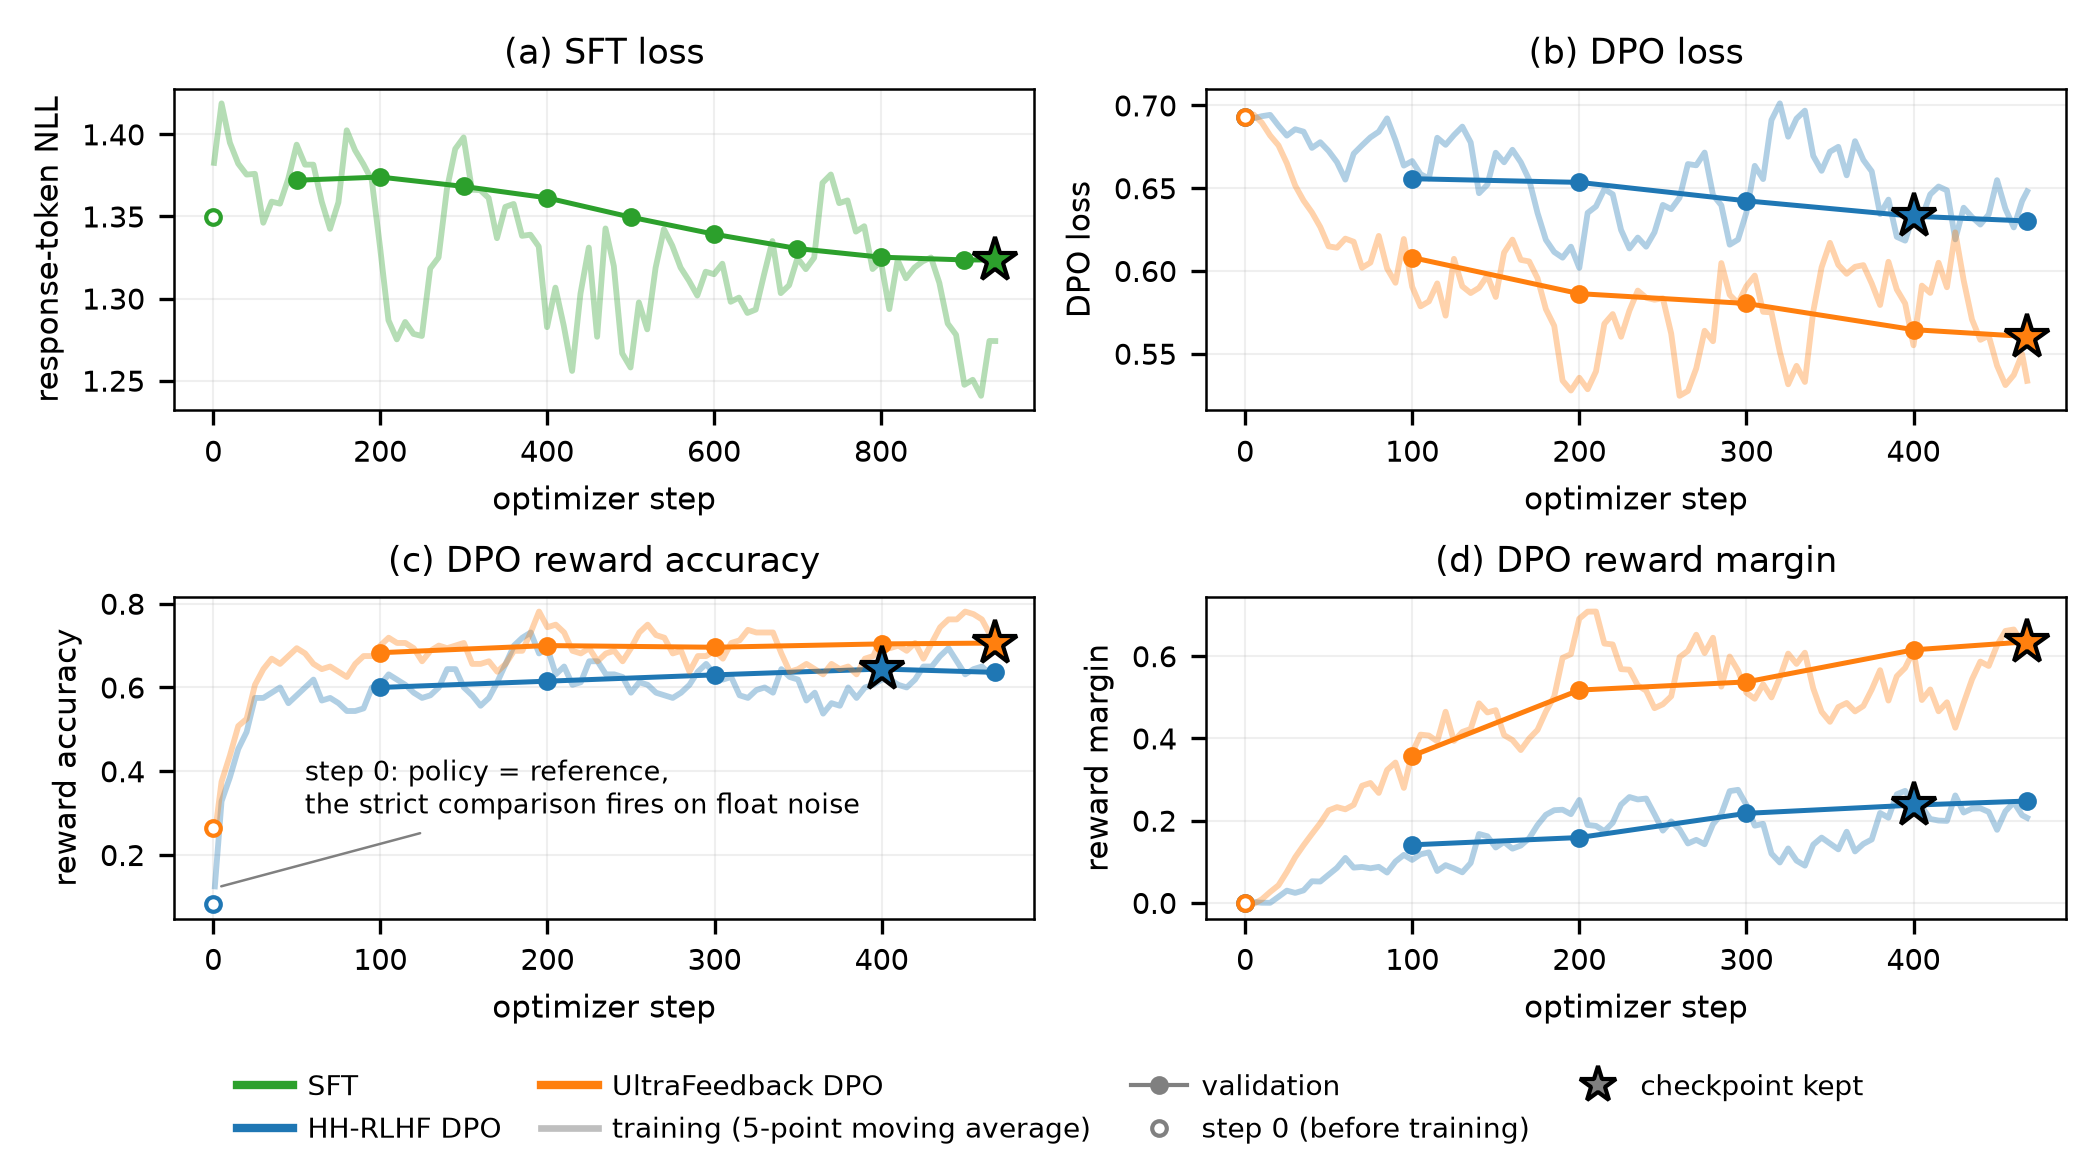
\includegraphics[width=0.84\textwidth]{assets/fig_training.png}
\caption{Training curves for SFT (a) and both DPO runs (b--d). Thin faded lines show training metrics, which I logged every 10 optimizer steps (SFT) or every 5 (DPO) and smoothed with a 5-point moving average. Dots show validation metrics at every 100 steps and at the last step. Hollow dots mark step 0, before any update, and stars mark the checkpoint I kept. In (c), the step-0 accuracy is an artifact: the policy equals the reference, so the two rewards differ only by floating-point noise.}
\label{fig:training}
\end{figure}

\paragraph{SFT.} Validation loss rose slightly from 1.350 at step 0 to 1.374 at step 200, then fell at every later evaluation to 1.323 at step 937 (perplexity 3.86 to 3.76). It never turned upward, so one epoch showed no sign of overfitting, and the best checkpoint is the final one. Training loss falls from a mean of 1.37 over the first ten logged steps to 1.28 over the last ten, and with one epoch every batch is new when I score it, so it behaves like a held-out loss.

\paragraph{DPO.} Both runs start at a loss of $\ln 2 \approx 0.693$, the value when the policy equals the reference. HH-RLHF improves slowly: validation loss falls from 0.656 at step 100 to 0.630 at the end, reward accuracy creeps from 0.60 to 0.64, and the reward margin grows from 0.14 to 0.25. UltraFeedback separates its pairs much more easily: validation loss falls from 0.608 to 0.560, accuracy rises from 0.68 to 0.71, and the margin grows from 0.36 to 0.63. Training and validation agree. Over the last 100 steps, training reward accuracy was 0.63 for HH-RLHF and 0.72 for UltraFeedback, against validation accuracies of 0.636 and 0.706, so I see no overfitting in either run. The UltraFeedback margin was still rising when the epoch ended, so that run had not converged.

\paragraph{Checkpoint selection.} I kept the checkpoint with the highest validation reward accuracy: step 400 (0.644) for HH-RLHF and the final step (0.706) for UltraFeedback. For HH-RLHF, step 400 beats the final step 468 (0.636) by only 0.8 points, which is less than the roughly 1.5-point binomial standard error of either number, and validation loss is marginally lower at step 468 (0.630 against 0.633). I therefore treat the two checkpoints as equivalent, and I see step 400 as a tie-break, not as evidence of overfitting.

\paragraph{Stability.} No run diverged. The only instability was fp16 overflow early in both DPO runs: the loss scaler halved three times, from 65,536 to 8,192, within the first 175 steps of each run, so I infer that it skipped three of the 468 updates in each run. SFT never overflowed.

\paragraph{Implicit rewards.} On the validation pairs, the implicit rewards of both the chosen and the rejected answers fell below zero in both runs (final values: $-0.30$ and $-0.55$ for HH-RLHF, $-0.12$ and $-0.75$ for UltraFeedback). The margin grows because the policy lowers the probability of rejected answers more than that of chosen ones, not because it raises the probability of chosen ones. Figure~\ref{fig:behavior}c and d plot both scores.

\paragraph{LoRA.} The LoRA run has only 39 updates on 198 pairs, too few for a curve. On its 22 validation pairs, the selected adapter reaches a reward accuracy of 1.0 and a margin of 0.96, which shows it separates the persona answer from the plain one, not that its generations change style.

None of these curves measures response quality. They show how well each model separates pairs from its own preference data, so I judge the checkpoints on generated responses, as the next section reports.
